\documentclass{article}%

\usepackage{amsmath}%
\usepackage{graphicx}
\usepackage[english,greek]{babel}
\usepackage[utf8x]{inputenc}
\usepackage{listings}
\usepackage{lipsum}

\newcommand{\exedout}{%
  \rule{0.8\textwidth}{0.5\textwidth}%
}



\begin{document}

\selectlanguage{greek}

\title{Δίκτυα Επικοινωνιών\\3η εργαστηριακή άσκηση}
\author{Γεώργιος Δασούλας\\Α.Μ: 03112010 \\ 6ο Εξάμηνο 2014-2015  }
\date{\today}
\maketitle

\textbf{{\underline{1.Μετάδοση δεδομένων σε δίκτυο με σύνθετη τοπολογία }}} \\

Σε αυτή την άσκηση θα ορίσουμε στο \textlatin{NS2} ένα δίκτυο που αποτελείται από
εννέα κόμβους και θα επιλέξουμε δύο κόμβους του δικτύου, που δεν συνδέονται άμεσα μεταξύ
τους, να ανταλλάσσουν δεδομένα. Με αυτό τον τρόπο θα παρατηρήσουμε πώς μεταβάλλεται η δρομολόγηση της ροής των δεδομένων μεταξύ κόμβων αποστολής και λήψης, ανάλογα με το πλήθος των κόμβων που παρεμβάλλονται , καθώς και τα κόστη ζεύξης μεταξύ των κόμβων.\\\\
Μετά την κατασκευή της τοπολογίας παρατηρούμε την παρακάτω μεταφορά δεδομένων. Στην τοπολογία έχουμε διακρίνει με διαφορετικό χρώμα τις δύο αποστολές δεδομένων με αντίθετη κατεύθυνση.Το παρακάτω στιγμιότυπο είναι σε χρόνο $0.7<t<3.7$ \textlatin{sec} , δηλαδή στο διάστημα που στέλνονται πακέτα και από τους δύο κόμβους 0,3.
\begin{figure}[htbp]
	\centering
		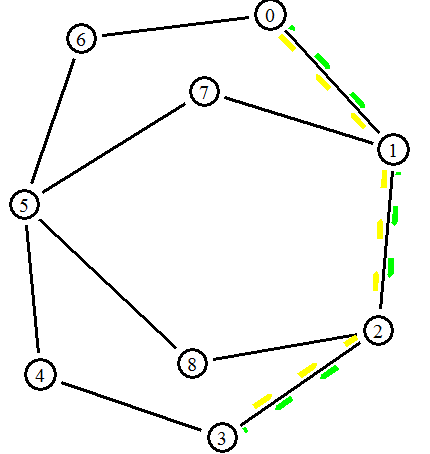
\includegraphics[width=0.30\textwidth]{1.png}
	\label{fig:1}
\end{figure}

\newpage


\textbf{\underline{Ερωτήσεις}} \\
\textsl{\textbf{{Απαντήσεις ερωτήσεων}}}

\begin{itemize}
\item Ποια διαδρομή ακολουθούν τα πακέτα $;$\\ 
\textbf{Απάντηση}:.Οπως φαίνεται στο παραπάνω \textlatin{animation} τα πακέτα ακολουθούν τη διαδρομή : 0 - 1 - 2 - 3 , καθώς και την αντίστροφη. 
\item Ελέγξτε αν η ροή των πακέτων και από τις δυο πλευρές ακολουθεί τη διαδρομή με τα
λιγότερα βήματα. \\
\textbf{Απάντηση}: Η ροή των πακέτων ακολουθεί τη διαδρομή με τους λιγότερους κόμβους - βήματα και επειδή οι ζεύξεις είναι αμφίδρομες ισχύει το ίδιο και για τις δύο πλευρές.
\item Υπάρχει συντομότερη διαδρομή από αυτήν που ακολουθούν, όσον αφορά τη συνολική
καθυστέρηση κάθε ροής $;$\\ 
\textbf{Απάντηση}:Όσον αφορά τη συνολική καθυστέρηση της ροής, δηλαδή το άθροισμα των καθυστερήσεων ζεύξεων (μιας και τα κόστη είναι ορισμένα μοναδιαία ακόμα) , η διαδρομή παραμένει η ελάχιστη με καθυστέρηση $40+40+40=120$ \textlatin{msec}. Όμως , ακόμα κι αν δεν ήταν η ελάχιστη καθυστέρηση πάλι η ίδια διαδρομή θα ακολουθούνταν , καθώς επιλέγεται με βάση το πλήθος των κόμβων - βημάτων.\\
\item Ποιος ο ρόλος των δύο παρακάτω εντολών $;$\selectlanguage{english}
 \begin{verbatim}$udp0 set packetSize_ 1500 ,
$udp3 set packetSize_ 1500 \end{verbatim} \selectlanguage{greek} Τι παρατηρείτε στις ροές των πακέτων αν αφαιρεθούν οι γραμμές
αυτές από τον κώδικα της προσομοίωσης;  $;$ \\
\textbf{Απάντηση}:  Οι δύο εντολές καθορίζουν το μέγιστο μήκος του πακέτου πληροφορίας που στέλνεται. Επομένως, εφόσον διαγραφούν οι δύο αυτές εντολές και κρατώντας σταθερό το μήκος πακέτου στα 1500 $bytes$ που θέλουμε να στείλουμε μέσω των γννητριών $CBR$ , θα πρέπει η πληροφορία να "σπάσει" σε δύο πακέτα, ένα των 1000 ( που είναι το προκαθορισμένο) και ένα των 500.Παρακάτω φαίνεται ακριβώς αυτή η διάσπαση:
\begin{center}
	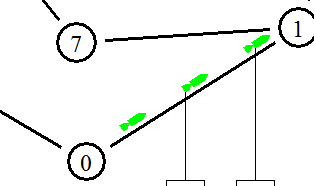
\includegraphics[width=0.30\textwidth]{2.png}
\end{center}

\end{itemize}

\textbf{{\underline{2. Στατική και δυναμική δρομολόγηση}}} \\\\
Εδώ θα δούμε τη διαφορά μεταξύ στατικής και δυναμικής δρομολόγησης, καθώς και το πώς το δίκτυο αντιμετωπίζει τις μεταβολές στην τοπολογία του. Για να δούμε αυτές τις διαφορές προσθέτουμε στην τοπολογία μας \textlatin{ protocol agents} που μπορούν να ενημερώνουν τους κόμβους σχετικά με την τοπολογία της παρούσας φάσης , καθιστώντας έτσι τη δρομολόγηση δυναμική.\\

\textbf{\underline{Ερωτήσεις}} \\
\textsl{\textbf{{Απαντήσεις ερωτήσεων}}}


\begin{itemize}
	\item Εξηγήστε γιατί, με τη στατική δρομολόγηση, οι κόμβοι εξακολουθούν να στέλνουν
πακέτα και μετά τη διακοπή της ζεύξης.\\ 
	\textbf{Απάντηση}: Αυτό συμβαίνει, διότι στη στατική δρομολόγηση οι κόμβοι που στέλνουν δεδομένα δε λαμβάνουν με κάποιο τρόπο πληροφορία για τη λειτουργικότητα των ζεύξεων.Γι΄ αυτό το λόγο , συνεχίζουν να στέλνουν πακέτα δεδομένων οι κόμβοι 0,3 τα οποία στη συνέχεια χάνονται. 
	\item Τα πακέτα που χάθηκαν, θα ξαναμεταδοθούν από τους αντίστοιχους κόμβους, όταν
επανέλθει η σύνδεση $;$ \\
	\textbf{Απάντηση}: Όχι, γιατί ακριβώς οι κόμβοι που στέλνουν δεδομένα δεν έχουν κάποια πληροφορία για το αν παραδόθηκαν τα πακέτα.
	\item Τι παρατηρείτε όταν γίνεται διακοπή ζεύξης και έχουμε δυναμική δρομολόγηση;
Περιγράψτε με απλά λόγια τη διαδικασία που λαμβάνει χώρα στο animation.Συμπίπτει η
αρχική με τη μόνιμη διαδρομή δρομολόγησης για τις δύο ροές κατά τη διάρκεια της
διακοπής $;$  \\
	\textbf{Απάντηση}: Αρχικά, τη στιγμή που διακόπτεται η ζεύξη 1,2 χάνονται τα πακέτα που βρίσκονται πάνω στη συγκεκριμένη ζεύξη, όπως επίσης και τα πακέτα που έρχονται από τις γειτονικές ζεύξεις προς αυτήν , έως ότου να ενημερωθούν από τους \textlatin{protocol agents} οι κόμβοι 1,2. Τη στιγμή που ενημερωθούν οι κόμβοι 1,2 τα πακέτα δεδομένων αλλάζουν ροή δρομολόγησης για τους προορισμούς τους και συγκεκριμένα ακολουθούν τις διαδρομές, έως ότου ενημερωθούν οι αρχικοί κόμβοι : $3 \rightarrow 2 \rightarrow 8 \rightarrow 5 \rightarrow 6 \rightarrow 0$ και $0 \rightarrow 1 \rightarrow 7 \rightarrow 5\rightarrow 4 \rightarrow 3$.Μόλις ενημερωθούν οι αρχικοί κόμβοι , τα πακέτα δεδομένων ακολουθούν τη μόνιμη διαδρομή , για όσο διάστημα έχουμε διακοπή της ζεύξης , δηλαδή τις διαδρομές : 0 - 6 - 5 - 4 - 3 και αντίστροφα.Παρακάτω, βρίσκονται δύο στιγμιότυπα μετά τη διακοπή της ζεύξης και πρίν την επαναφορά της.
	\begin{figure}[htbp]
\centering
\begin{minipage}{0.33\textwidth}
\centering
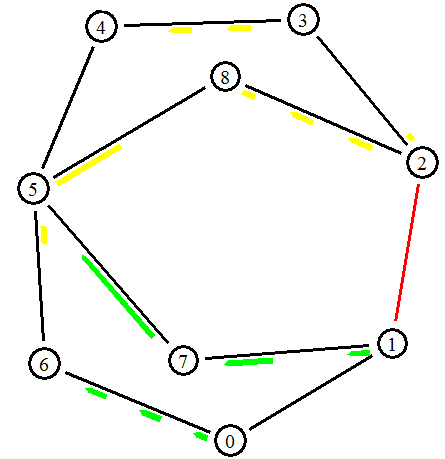
\includegraphics[width=1.00\textwidth]{4.png}
\caption{α) Μεταβατική κατάσταση}
\end{minipage}\hfill
\begin{minipage}{0.35\textwidth}
\centering
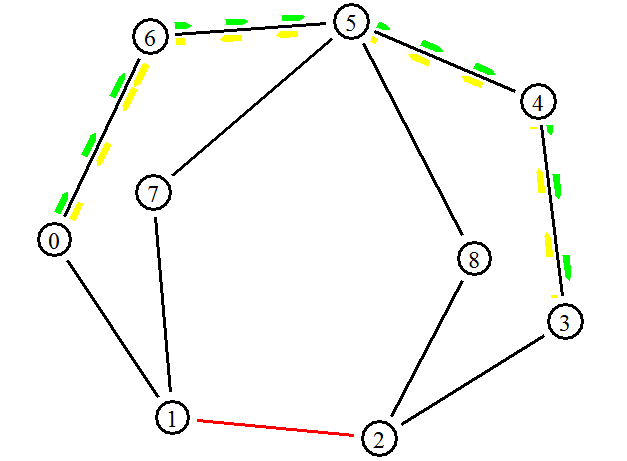
\includegraphics[width=1.00\textwidth]{3.png}
\caption{β) Μόνιμη διαδρομή}
\end{minipage}
\end{figure}
	\item Με βάση το \textlatin{animation}, προσδιορίστε για κάθε ροή τη χρονική στιγμή όπου παρατηρείται
η μόνιμη διαδρομή δρομολόγησης κατά τη διάρκεια διακοπής.\\
	\textbf{Απάντηση}: Από το \textlatin{animation} παρατηρούμε πως η κάθε ροή ακολουθεί σχεδόν ταυτόχρονα την μόνιμη διαδρομή δρομολόγησης , η οποία είναι κοινή και για τις δύο ροές περίπου στη χρονική στιγμή $t=1.85$ $sec$. Αυτός ο χρόνος εξαρτάται από την ταχύτητα με την οποία οι $rtproto$ $agents$ θα ενημερώσουν τους κόμβους.
	\item Για ποιο λόγο τα πακέτα ακολουθούν τις συγκεκριμένες διαδρομές αφότου πέσει η
σύνδεση, στην αρχική και τη μόνιμη κατάσταση $;$ \\
	\textbf{Απάντηση}: Όπως εξηγήθηκε παραπάνω , αυτό οφείλεται στο ποιοί κόμβοι είναι κάθε στιγμή ενημερωμένοι για την τοπολογία του δικτύου.Αρχικά, εφόσον διακοπεί η ζεύξη μεταξύ των 1,2 και χαθούν τα πακέτα που είναι εκείνη τη στιγμή πάνω στη ζεύξη, ενημερώνονται οι κόμβοι 1,2 για την αλλαγή της τοπολογίας. Οπότε, τα πακέτα δρομολογούνται μέσω των ζεύξεων 2-8 και 1-7 αντίστοιχα. Στη συνέχεια , ενημερώνονται και οι κόμβοι 3,0 και έτσι επιλέγεται άλλη διαδρομή, η οποία είναι και η μόνιμη δρομολόγηση για το διάστημα που έχουμε διακοπή της ζεύξης.
	\item Θα μπορούσαν να δρομολογηθούν από άλλους κόμβους $;$\\
	\textbf{Απάντηση}: Υπάρχουν και άλλες δυνατές ροές δρομολόγησης που δεν περιλαμβάνουν τη ζεύξη 1-2 ( όπως π.χ : 3-2-8-5-7-1-0) , αλλά δεν είναι οι ελάχιστες.
	\item Ποιος από όλους τους κόμβους καθορίζει από ποια διαδρομή θα προωθηθούν κάθε φορά
τα πακέτα $; $\\ 
	\textbf{Απάντηση}: Οι ενημερωμένοι σχετικά με την τοπολογία κόμβοι , οι οποίοι προηγούνται των πακέτων που στέλνονται είναι αυτοί που καθορίζουν τη διαδρομή, όταν οι πηγές δεν είναι ακόμα σε θέση ( μέχρι να ενημερωθούν) να ορίσουν την ελάχιστη διαδρομή.
	
	
\end{itemize}

\textbf{{\underline{3. Καθορισμός κόστους ζεύξης}}} \\\\
Στη συγκεκριμένη ενότητα θα μεταβάλλουμε το κόστος της ζεύξης για να δούμε πως καθορίζουν αυτές οι αλλαγές την επιλογή της ελάχιστης ροής δρομολόγησης των πακέτων. Συγκεκριμένα, μέχρι στιγμής είχαμε προκαθορισμένα μοναδιαίο κόστος στις ζεύξεις μεταξύ των κόμβων. Τώρα, θα ορίσουμε τα κόστη των ζεύξεων ανάλογα των καθυστερήσεων.\\\\

\newpage

\textbf{\underline{Ερωτήσεις}} \\
\textsl{\textbf{{Απαντήσεις ερωτήσεων}}}
\begin{itemize}
	\item Ποιες διαδρομές ακολουθούν τα πακέτα πριν, κατά τη διάρκεια και μετά την πτώση της
σύνδεσης για τις δύο ροές $;$ \\
\textbf{Απάντηση}: Πριν την πτώση της ζεύξης 1-2 η διαδρομή που ακολουθείται και από τις δύο ροές δεδομένων είναι ίδια με πριν, δηλαδή η 0-1-2-3 και αντίστροφα. Μετά την πτώση της ζεύξης οι αρχικές διαδρομές είναι οι : $0\rightarrow1\rightarrow 7\rightarrow 5\rightarrow 4\rightarrow 3$ (για τα πακέτα που στέλνονται από τον κόμβο 0) και $ 3\rightarrow 2\rightarrow 8\rightarrow 5\rightarrow 7\rightarrow 1\rightarrow 0$ (για τα πακέτα που στέλνονται από τον κόμβο 3). Οι μόνιμες διαδρομές μετά την πτώση της ζεύξης και πριν την επαναφορά της είναι οι εξής : $0\rightarrow1\rightarrow 7\rightarrow 5\rightarrow 4\rightarrow 3$ (για τα πακέτα που στέλνονται από τον κόμβο 0), η οποία παρέμεινε ίδια και $3\rightarrow 4\rightarrow 5\rightarrow 7\rightarrow 1\rightarrow 0$ (για τα πακέτα που στέλνονται από τον κόμβο 3). Παρακάτω , φαίνονται οι τρεις καταστάσεις :
\begin{figure}[htbp]
\centering
\begin{minipage}{0.36\textwidth}
\centering
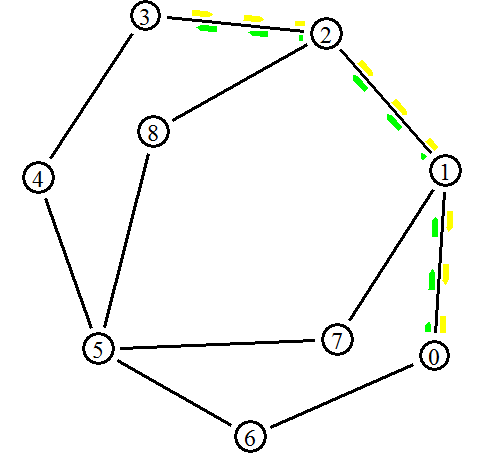
\includegraphics[width=1.00\textwidth]{6.png}
\caption{α) Πριν την πτώση ζεύξης}
\end{minipage}\hfill
\begin{minipage}{0.35\textwidth}
\centering
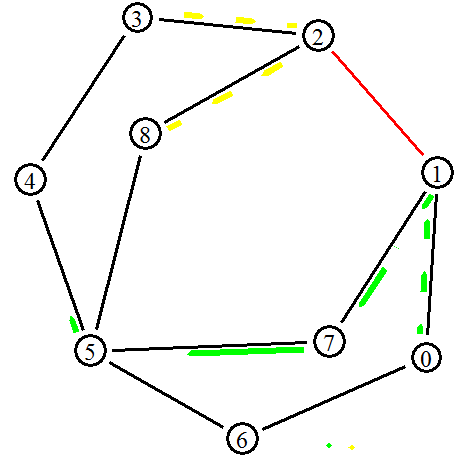
\includegraphics[width=1.00\textwidth]{7.png}
\caption{β) Αρχική διαδρομή μετά την πτώση}
\end{minipage}
\begin{minipage}{0.35\textwidth}
\centering
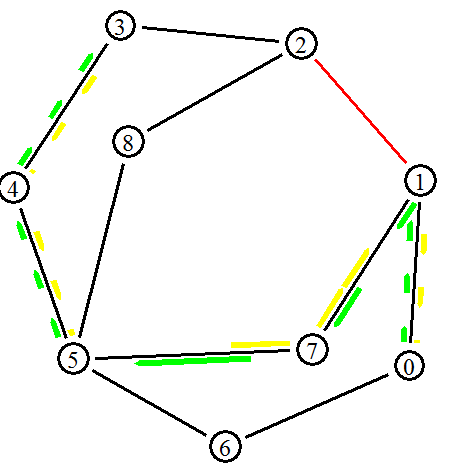
\includegraphics[width=1.00\textwidth]{8.png}
\caption{β) Μόνιμη διαδρομή μετά την πτώση}
\end{minipage}

\end{figure}

\item Για ποιον λόγο τα πακέτα ακολουθούν τις συγκεκριμένες διαδρομές $;$\\ 
\textbf{Απάντηση}: Πριν την πτώση ζεύξης είχαμε τη διαδρομή 0-1-2-3 , γιατί η συνολική καθυστέρηση της διαδρομής , η οποία καθορίζει και το αντίστοιχο κόστος ήταν η ελάχιστη και ίση με 120 $ms$. Μετά την πτώση της ζεύξης , η διαδρομή που τελικά προτιμάται έχει και πάλι την ελάχιστη πλέον καθυστέρηση ζεύξης που ισούται με 150 $ms$.
\item Θα μπορούσαν να δρομολογηθούν από άλλους κόμβους $;$\\ 
\textbf{Απάντηση}:Υπάρχουν και άλλες δυνατές ροές δρομολόγησης που δεν περιλαμβάνουν τη ζεύξη 1-2 , όπως και την περίπτωση που είχαμε μοναδιαία κόστη , αλλά δεν είναι οι ελάχιστες.
\item Μετά την αποκατάσταση της ζεύξης μεταξύ των κόμβων “1” και “2”, προσδιορίστε με
βάση το \textlatin{animation} τη χρονική στιγμή όπου παρατηρείται η μόνιμη διαδρομή
δρομολόγησης για κάθε ροή. \\
\textbf{Απάντηση}: Μετά την αποκάτασταση της ζεύξης, η μόνιμη διαδρομή δρομολόγησης προτιμάται περίπου στα 2.8 $sec$.
\item Ποιος είναι ο ρόλος της παρακάτω εντολής $;$ \selectlanguage{english}\begin{verbatim}Agent/rtProto/Direct set preference_ 200 \end{verbatim} \selectlanguage{greek}
Τι παρατηρείτε στη δρομολόγηση των πακέτων αν αφαιρεθεί η εντολή αυτή από τον
κώδικα της προσομοίωσης $;$ Αιτιολογείστε γιατί συμβαίνει αυτό. \\
\textbf{Απάντηση}: Ο ρόλος αυτής της εντολής σε συνδυασμό με τη στρατηγική $DV$ είναι να δίνει τη δυνατότητα στον $agent$ να ενημερώνεται σχετικά με την συνδεσμολογία της τοπολογίας, καθώς και να υπολογίζει τις ταχύτερες διαδρομές. Η $Direct$ κρατάει μόνο τις καταστάσεις των διπλανών κόμβων , που συνδεόνται άμεσα με τον παρόντα κόμβο , ενώ η $DV$ κρατάει σε κάθε κόμβο τις καταστάσεις όλης της τοπολογίας. Γι' αυτό αν εφαρμόσουμε την $DV$ περίσσοτερο από την $Direct$ θα δούμε να ενημέρωνονται λίγο πιο αργά οι κόμβοι για την ταχύτερη και λειτουργική διαδρομή.Αν αφαιρέσουμε την εντολή , τότε το $preference$ του $Direct$ παίρνει την προκαθορισμένη του τιμή , με συνέπεια να εφαρμόζεται περισσότερο αυτό το πρωτόκολλο και έτσι να έχουμε λίγο ταχύτερη δρομολόγηση.\end{itemize}


\textbf{{\underline{4. Παρακολούθηση εκθετικής κίνησης με το \textlatin{Xgraph}}}} \\\\

\begin{figure}[htbp]
\centering
\begin{minipage}{0.49\textwidth}
\centering
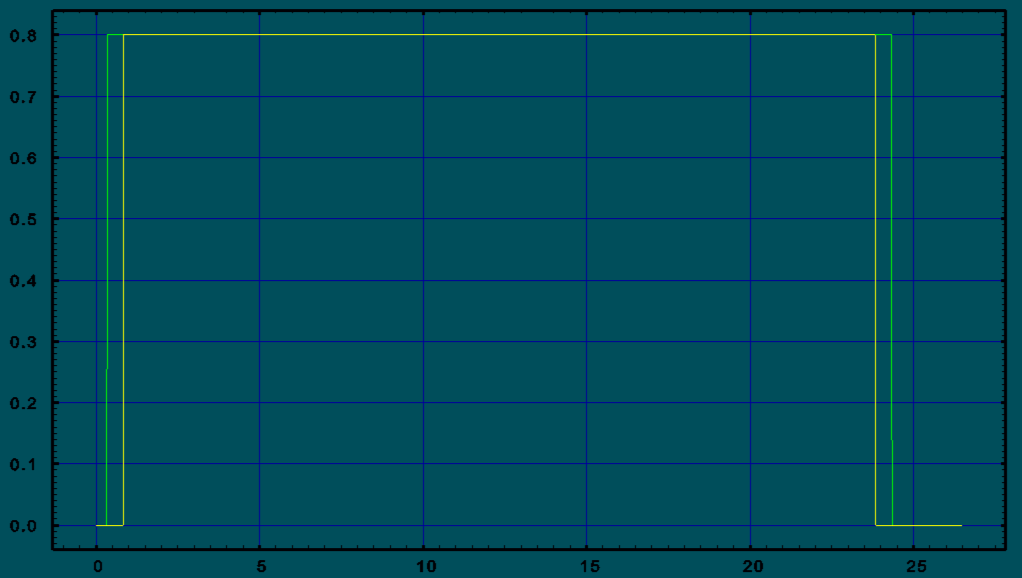
\includegraphics[width=1.00\textwidth]{9.png}
\caption{α) $CBR$ κίνηση}
\end{minipage}\hfill
\begin{minipage}{0.49\textwidth}
\centering
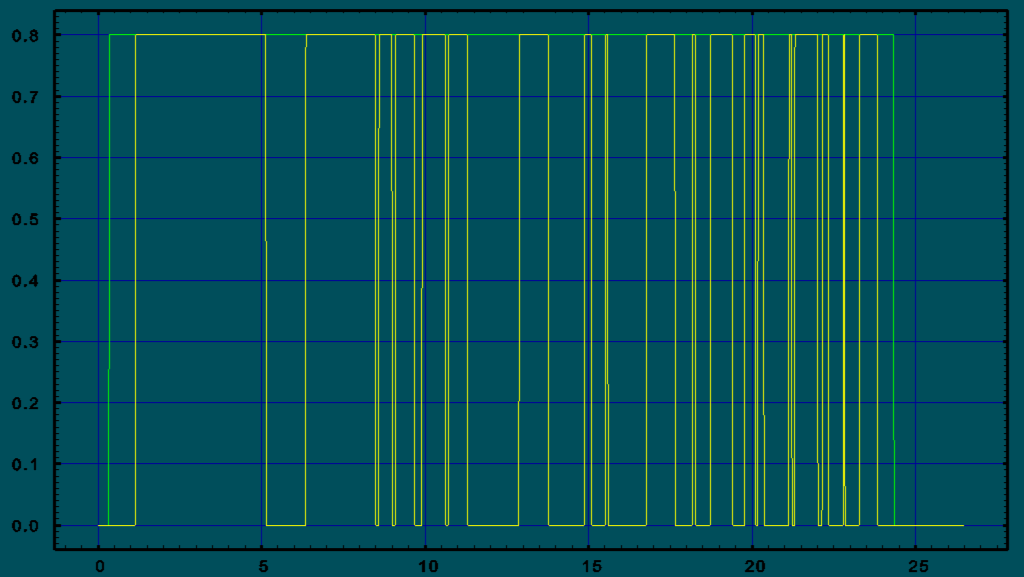
\includegraphics[width=1.00\textwidth]{10.png}
\caption{β) Εκθετική κίνηση}
\end{minipage}
\end{figure}

\textbf{\underline{Ερωτήσεις}} \\
\textsl{\textbf{{Απαντήσεις ερωτήσεων}}}
\begin{itemize}
	\item Ποιος είναι ο μέγιστος ρυθμός μετάδοσης που επιτυγχάνεται για τις δύο περιπτώσεις
κίνησης, βάσει των γραφικών παραστάσεων που σχεδιάσατε $;$\\
	\textbf{Απάντηση}: Όπως βλέπουμε από τα διαγράμματα , ο μέγιστος ρυθμός μετάδοσης είναι κοινός για τους δύο τύπους κίνησης και είναι ίσος με 0.8 $Mbits/sec$.
	\item Αιτιολογείστε τις μέγιστες τιμές που προσδιορίσατε παραπάνω, χρησιμοποιώντας τις
παραμέτρους που θέσατε για τη διαμόρφωση των δύο πηγών κίνησης ($CBR$ και
\textlatin{Exponential}). \\
	\textbf{Απάντηση}: Για τη $CBR$ κίνηση , από τις παραμέτρους που έχουμε θέσει προκύπτει ως μέγιστος ρυθμός μετάδοσης : $ \frac{packetSize}{interval}= \frac{1500 bytes}{0.015 sec}=100.000$ $bytes/sec$ =800.000 $bits/sec$ = 781.25 $Kbits/sec$. Για την εκθετική κίνηση ορίζεται άμεσα μέσω της παραμέτρου $rate$ ο ρυθμός μετάδοσης που είναι ίσος με $800Kbits/sec$. Και στις δύο περιπτώσεις κινήσεων βλέπουμε πως συγκλίνουν οι τιμές που υπολογίσαμε με τις παρατηρήσεις μας από τα διαγράμματα.
	\item Υπολογίστε το πλήθος των \textlatin{bytes} που λαμβάνονται επιτυχώς στον προορισμό για κάθε
ροή, θεωρώντας ότι και οι δύο ροές ολοκληρώνονται σε χρόνο $t=20+(a/10)$ $sec$, όπου $a$ τα
δύο τελευταία ψηφία του αριθμού μητρώου σας. \\
	\textbf{Απάντηση}: Για τη συγκεκριμένη εργασία έχουμε : $t=20+(10/10)=21$ $sec$. Κάνοντας κατάλληλες τροποποιήσεις στον κώδικάς μας , ώστε να υπολογίζει το συνολικό μέτρημα των $bytes$ για κάθε ροή έχουμε : για τη ροή $0\rightarrow 3$ : 2.080.500 $bytes$  και για τη ροή $3\rightarrow 0$ είναι 1.179.000 $bytes$. Μάλιστα, για τη $CBR$ κίνηση μπορούμε να μετρήσουμε το εμβαδό από το γράφημα και να δούμε ότι συγκλίνουν τα αποτελέσματά μας. (εμβαδό = $0.8$ $MBits/sec$$*21 sec = 2.202.009$). \\
Οι τροποποιήσεις που κάναμε φαίνονται στον ακόλουθο κώδικα :

\selectlanguage{english}

\begin{verbatim}
set ns [new Simulator]
set nf [open lab3a.nam w]
$ns namtrace-all $nf
set f0 [open out0.tr w]
set f3 [open out3.tr w]
set sum0 0
set sum3 0
proc record {} {
	global sink0 sink3 f0 f3 sum0 sum3
	set ns [Simulator instance]
	set time 0.015
	set sum0 [expr [$sink3 set bytes_] + $sum0]
	set sum3 [expr [$sink0 set bytes_] + $sum3]
	set bw0 [$sink3 set bytes_]
	set bw3 [$sink0 set bytes_]
	set now [$ns now]
	puts $f0 "$now [expr (($bw0/$time)*8)/1000000]"
	puts $f3 "$now [expr (($bw3/$time)*8)/1000000]"
	$sink0 set bytes_ 0
	$sink3 set bytes_ 0
	$ns at [expr $now +$time] "record"
}
for {set i 0} {$i < 9} {incr i}	{
	set n($i) [$ns node]
} 	
for {set i 0} {$i<7} {incr i}	{
	$ns duplex-link $n($i) $n([expr ($i+1)%7]) 2Mb 40ms DropTail
}
$ns duplex-link $n(7) $n(1) 2Mb 20ms DropTail
$ns duplex-link $n(7) $n(5) 2Mb 10ms DropTail
$ns duplex-link $n(8) $n(5) 2Mb 10ms DropTail
$ns duplex-link $n(8) $n(2) 2Mb 40ms DropTail
proc finish	{}	{
	global ns nf f0 f3 sum0 sum3
	$ns flush-trace
	close $nf
	close $f0
	close $f3
	puts $sum0
	puts $sum3
	exit 0
}
set udp0 [new Agent/UDP]
$udp0 set packetSize_ 1500
$ns attach-agent $n(0) $udp0
$udp0 set fid_ 0
$ns color 0 green
set sink0 [new Agent/LossMonitor]
$ns attach-agent $n(0) $sink0
set udp3 [new Agent/UDP]
$udp3 set packetSize_ 1500
$ns attach-agent $n(3) $udp3
$udp3 set fid_ 3
$ns color 3 yellow
set sink3 [new Agent/LossMonitor]
$ns attach-agent $n(3) $sink3
$ns connect $udp0 $sink3
$ns connect $udp3 $sink0
set cbr0 [new Application/Traffic/CBR]
$cbr0 set packetSize_ 1500
$cbr0 set interval_ 0.015
$cbr0 attach-agent $udp0
set Exponential3 [new Application/Traffic/Exponential]
$Exponential3 set packetSize_ 1500
$Exponential3 set rate_ 800k
$Exponential3 attach-agent $udp3
$ns at 0.0 "record"
$ns at 0.2 "$cbr0 start"
$ns at 0.7 "$Exponential3 start"
$ns at 21 "$Exponential3 stop"
$ns at 21 "$cbr0 stop"
$ns at 22 "finish"
$ns run


\end{verbatim} 
	
	
\end{itemize}


\end{document}